\begin{frame}{DAG LCA(33851)}

무가중치 방향 비순환 그래프 $G$가 주어진다. 다음 쿼리를 수행하는 프로그램을 작성하시오.

$u$ $v$: 두 정점 $u$와 $v$로 가는 경로가 모두 존재하는 모든 정점에 대해 $u$와 $v$로 가는 두 최단 경로의 길이 중 작지 않은 값의 최솟값을 출력한다. 두 정점 $u$와 $v$로 가는 경로가 존재하는 정점이 없다면 대신 -1을 출력한다.

첫 번째 줄에 그래프 $G$의 정점의 개수 $n$, 간선의 개수 $m$, 질의의 개수 $q$가 공백으로 구분되어 주어진다. ($5 \leq n \leq 2\,000; 0 \leq m \leq 4\,000; 1 \leq q \leq 1\,000$)

두 번째 줄부터 $m$개의 줄에 걸쳐 간선으로 연결된 두 정점의 번호 $u$, $v$가 한 줄에 하나씩 주어진다. 이는 $u$에서 $v$로 향하는 방향의 간선을 의미한다. ($1 \leq u, v \leq n; u \neq v$)

$m+2$번째 줄부터 $q$개의 줄에 걸쳐 쿼리가 한 줄에 하나씩 주어진다.

\end{frame}

\begin{frame}{예제 방향 그래프와 쿼리}

\centering

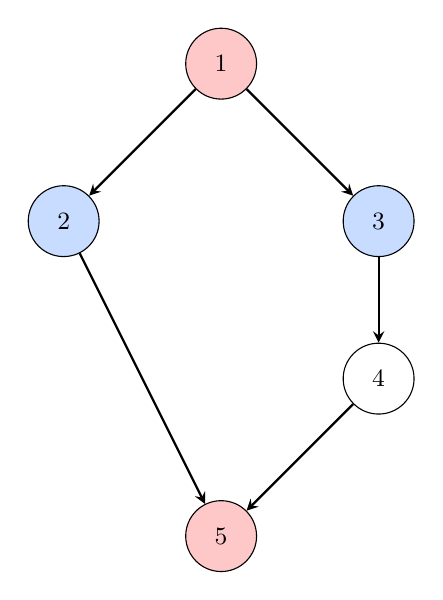
\begin{tikzpicture}[
    every node/.style={
        circle,
        draw,
        minimum size=9mm,
        font=\small
    }
]

% 색 정의
\definecolor{queryA}{RGB}{255,200,200} % (1,5) 빨강 계열
\definecolor{queryB}{RGB}{200,220,255} % (2,3) 파랑 계열

% 노드 (쿼리별 색칠)
\node[fill=queryA] (1) at (0,0) {1};

\node[fill=queryB] (2) at (-2,-2) {2};
\node[fill=queryB] (3) at (2,-2) {3};

\node (4) at (2,-4) {4};

\node[fill=queryA] (5) at (0,-6) {5};

% 간선
\draw[->, thick, >=stealth] (1) -- (2);
\draw[->, thick, >=stealth] (2) -- (5);

\draw[->, thick, >=stealth] (1) -- (3);
\draw[->, thick, >=stealth] (3) -- (4);
\draw[->, thick, >=stealth] (4) -- (5);

\vspace{2mm}

\end{tikzpicture}

\end{frame}

\begin{frame}{간선의 방향을 뒤집은 그래프 $G^T$}

\centering

\begin{minipage}{0.45\textwidth}
\centering
\textbf{$G$}

\vspace{3mm}

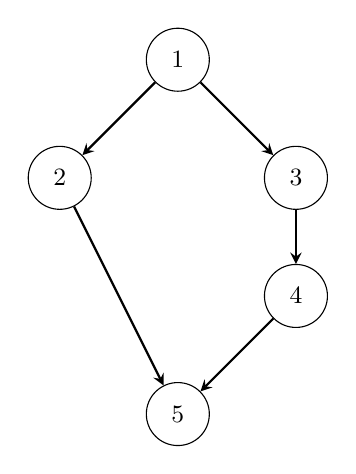
\begin{tikzpicture}[
    every node/.style={
        circle,
        draw,
        minimum size=8mm,
        font=\small
    }
]

% 노드
\node (1) at (0,0) {1};
\node (2) at (-1.5,-1.5) {2};
\node (3) at (1.5,-1.5) {3};
\node (4) at (1.5,-3) {4};
\node (5) at (0,-4.5) {5};

% 간선 (원본)
\draw[->, thick, >=stealth] (1) -- (2);
\draw[->, thick, >=stealth] (2) -- (5);

\draw[->, thick, >=stealth] (1) -- (3);
\draw[->, thick, >=stealth] (3) -- (4);
\draw[->, thick, >=stealth] (4) -- (5);

\end{tikzpicture}

\end{minipage}
\hfill
\begin{minipage}{0.45\textwidth}
\centering
\textbf{$G^T$}

\vspace{3mm}

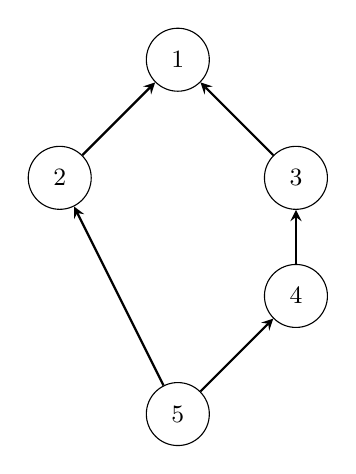
\begin{tikzpicture}[
    every node/.style={
        circle,
        draw,
        minimum size=8mm,
        font=\small
    }
]

% 노드 (같은 위치)
\node (1) at (0,0) {1};
\node (2) at (-1.5,-1.5) {2};
\node (3) at (1.5,-1.5) {3};
\node (4) at (1.5,-3) {4};
\node (5) at (0,-4.5) {5};

% 간선 (뒤집힘)
\draw[->, thick, >=stealth] (2) -- (1);
\draw[->, thick, >=stealth] (5) -- (2);

\draw[->, thick, >=stealth] (3) -- (1);
\draw[->, thick, >=stealth] (4) -- (3);
\draw[->, thick, >=stealth] (5) -- (4);

\end{tikzpicture}

\end{minipage}

\end{frame}

\setproblem{33851}

% \begin{frame}[fragile, allowframebreaks]{김준형 소스 코드}
% \inputminted{java}{\prob/Junhyeong.java}
% \end{frame}

\begin{frame}[fragile, allowframebreaks]{정의찬 소스 코드}
\inputminted{java}{\prob/Uichan.java}
\end{frame}

\begin{frame}[fragile, allowframebreaks]{서민종(구) 소스 코드}
\inputminted{java}{\prob/MinjongOld.java}
\end{frame}

\begin{frame}[fragile, allowframebreaks]{서민종(신) 소스 코드}
\inputminted{java}{\prob/MinjongNew.java}
\end{frame}

\begin{frame}[fragile, allowframebreaks]{원찬혁 소스 코드}
\inputminted{java}{\prob/Chanhyeok.java}
\end{frame}

\begin{frame}[fragile, allowframebreaks]{손현준 소스 코드}
\inputminted{java}{\prob/Hyeonjun.java}
\end{frame}

\begin{frame}[fragile, allowframebreaks]{김지훈 소스 코드}
\inputminted{java}{\prob/Jihoon.java}
\end{frame}

\begin{frame}[fragile, allowframebreaks]{김시온 소스 코드}
\inputminted{java}{\prob/Sion.java}
\end{frame}

\begin{frame}[fragile, allowframebreaks]{임건애 소스 코드}
\inputminted{java}{\prob/Keonae.java}
\end{frame}